\chapter{Threshold voltages of the PMTs}
\label{sec:appendix}
\begin{figure}
    \centering
    \begin{subfigure}[b]{0.48\textwidth}
    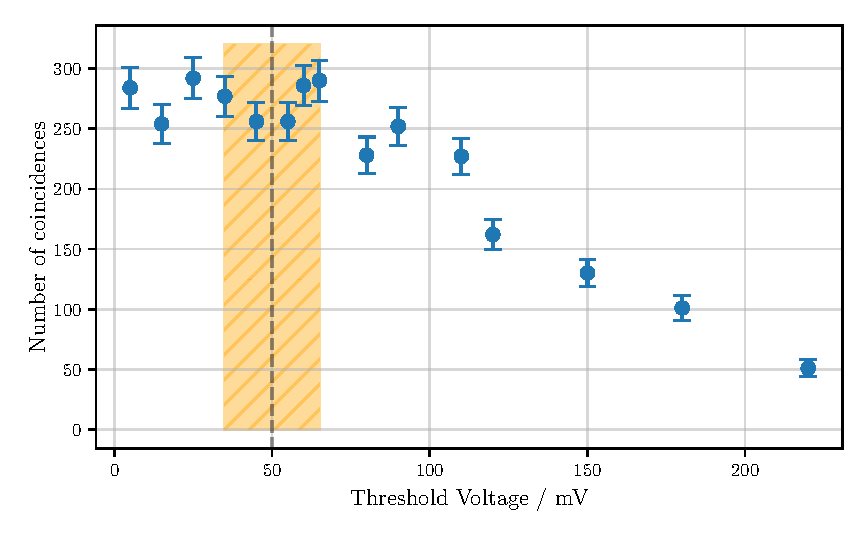
\includegraphics[width=\textwidth]{plots/threshR00.pdf}
    \captionof{figure}{Data of the \texttt{R00} signal.
    The central value of the plateau is $\SI{50}{mV}$.}
\end{subfigure}\hfill
\begin{subfigure}[b]{0.48\textwidth}
    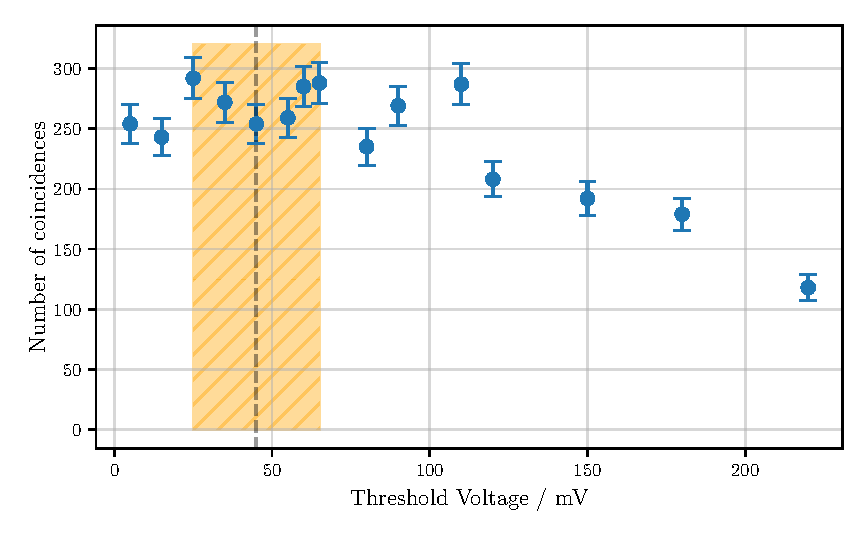
\includegraphics[width=\textwidth]{plots/threshR10_2.pdf}
    \captionof{figure}{Data of the second measurement of the \texttt{R10} signal.
    The central value of the plateau is $\SI{45}{mV}$.}
\end{subfigure}
\caption{Measured number of coincidences concerning varying threshold voltages
of the \texttt{R00} and \texttt{R10} PMTs.
The dashed line indicates the central values of each plateau. The striped orange areas mark the found plateaus.}
\label{fig:appthresh1}
\end{figure}
\begin{figure}
    \begin{subfigure}[b]{0.48\textwidth}
        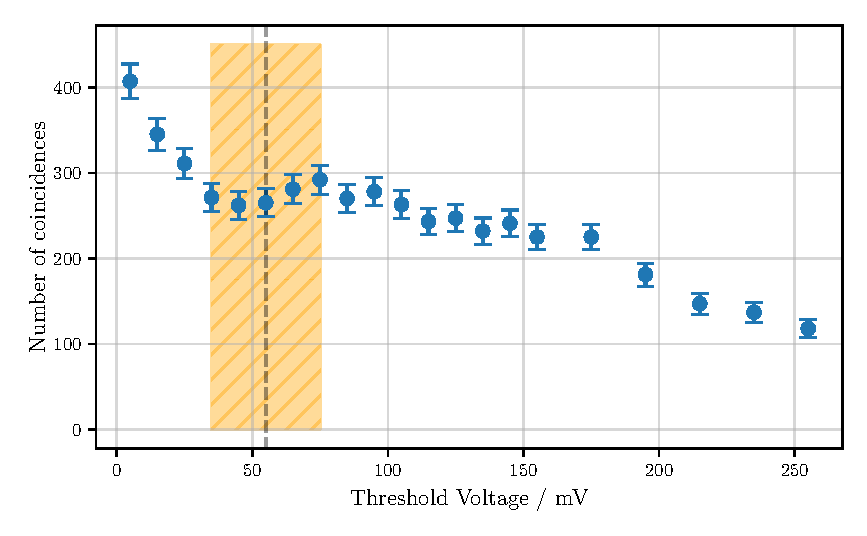
\includegraphics[width=\textwidth]{plots/threshR01.pdf}
        \captionof{figure}{Data of the \texttt{R01} PMTs.
        The central value of the plateau is $\SI{55}{mV}$.}
    \end{subfigure}\hfill
    \begin{subfigure}[b]{0.48\textwidth}
        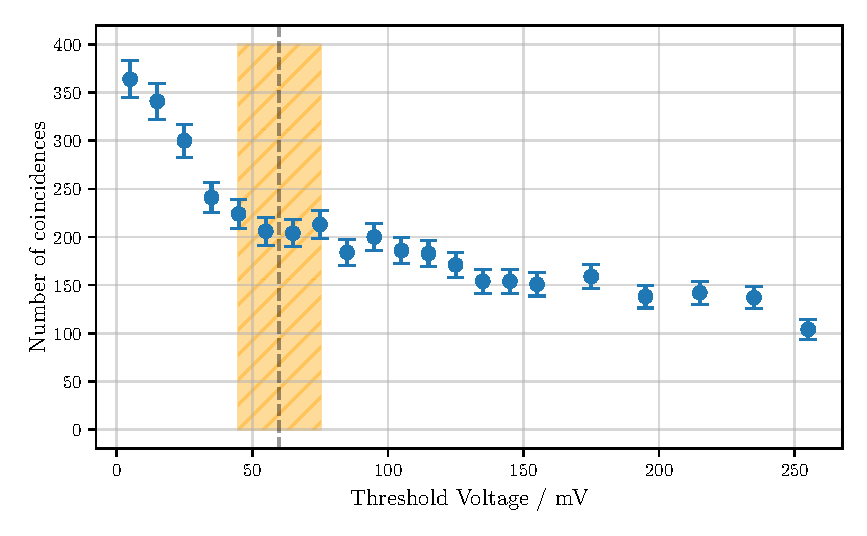
\includegraphics[width=\textwidth]{plots/threshR11.pdf}
        \captionof{figure}{Data of the \texttt{R11} PMTs.
        The central value of the plateau is $\SI{60}{mV}$.}
    \end{subfigure}
    \caption{Measured number of coincidences concerning varying threshold voltages
    of the \texttt{R01} and \texttt{R11} PMTs.
    The dashed line indicates the central values of each plateau. The striped orange areas mark the found plateaus.}
    \label{fig:appthresh2}
\end{figure}   
\begin{figure}
    \centering
    \begin{subfigure}[b]{0.48\textwidth}
        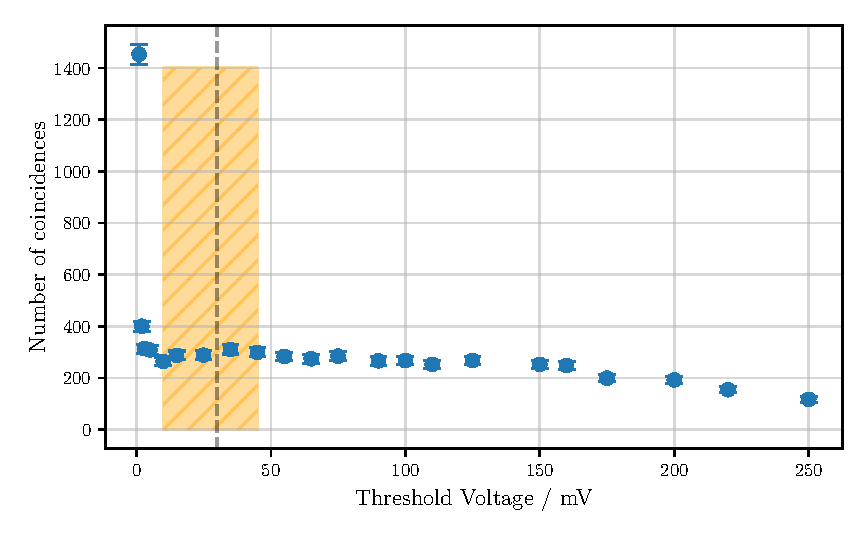
\includegraphics[width=\textwidth]{plots/threshL00.pdf}
        \captionof{figure}{Data of the \texttt{L00} PMTs.
        The central value of the plateau is $\SI{30}{mV}$.}
    \end{subfigure}\hfill
    \begin{subfigure}[b]{0.48\textwidth}
        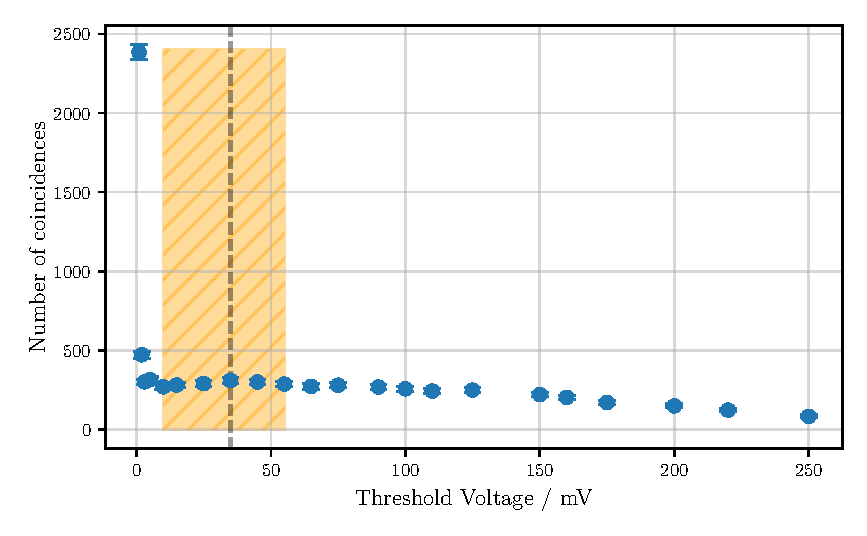
\includegraphics[width=\textwidth]{plots/threshL10.pdf}
        \captionof{figure}{Data of the \texttt{L10} PMTs.
        The central value of the plateau is $\SI{35}{mV}$.}
    \end{subfigure}
    \caption{Measured number of coincidences concerning varying threshold voltages
    of the \texttt{L00} and \texttt{L10} PMTs.
    The dashed line indicates the central values of each plateau. The striped orange areas mark the found plateaus.}
    \label{fig:appthresh3}
\end{figure}
\begin{figure}
    \centering
    \begin{subfigure}[b]{0.48\textwidth}
        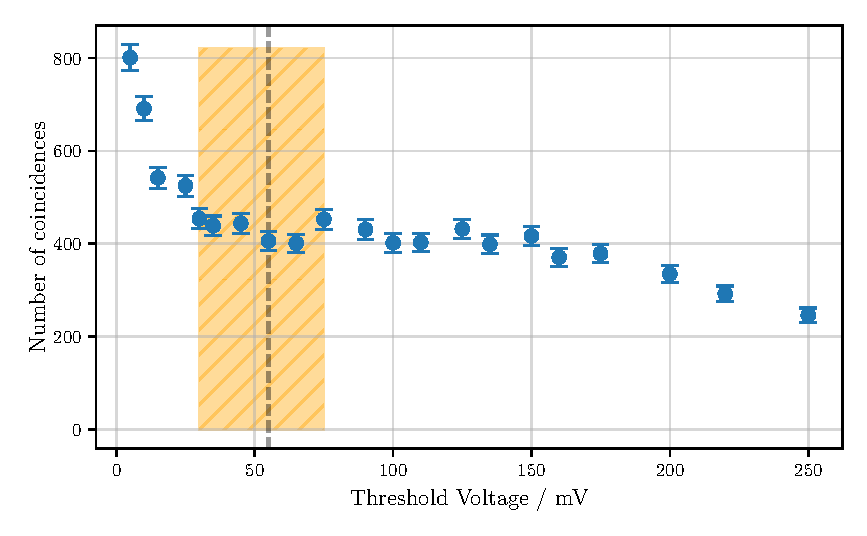
\includegraphics[width=\textwidth]{plots/threshL01.pdf}
        \captionof{figure}{Data of the \texttt{L01} PMTs.
        The central value of the plateau is $\SI{55}{mV}$.}
    \end{subfigure}\hfill
    \begin{subfigure}[b]{0.48\textwidth}
        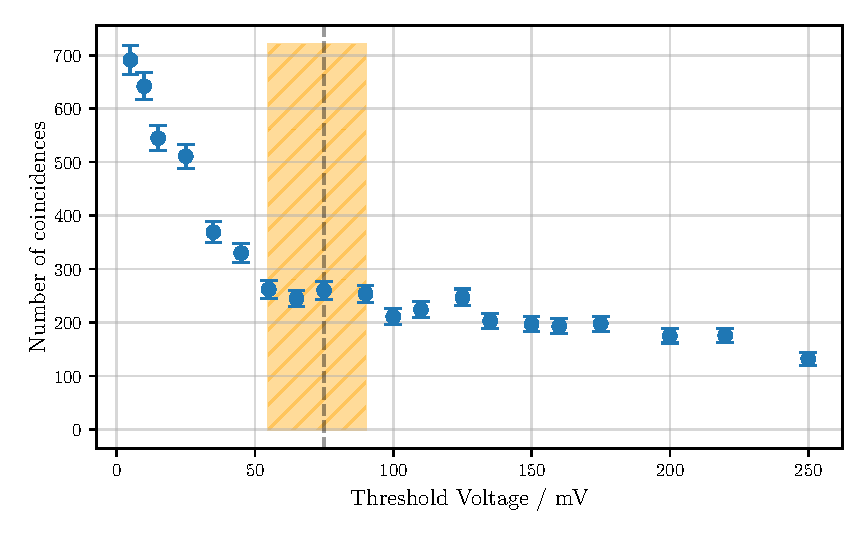
\includegraphics[width=\textwidth]{plots/threshL11.pdf}
        \captionof{figure}{Data of the \texttt{L11} PMTs.
        The central value of the plateau is $\SI{75}{mV}$.}
    \end{subfigure}
    \caption{Measured number of coincidences concerning varying threshold voltages
    of the \texttt{L01} and \texttt{L11} PMTs.
    The dashed line indicates the central values of each plateau. The striped orange areas mark the found plateaus.}
    \label{fig:appthresh4}
\end{figure}
\begin{figure}
    \centering
    \begin{subfigure}[b]{0.48\textwidth}
        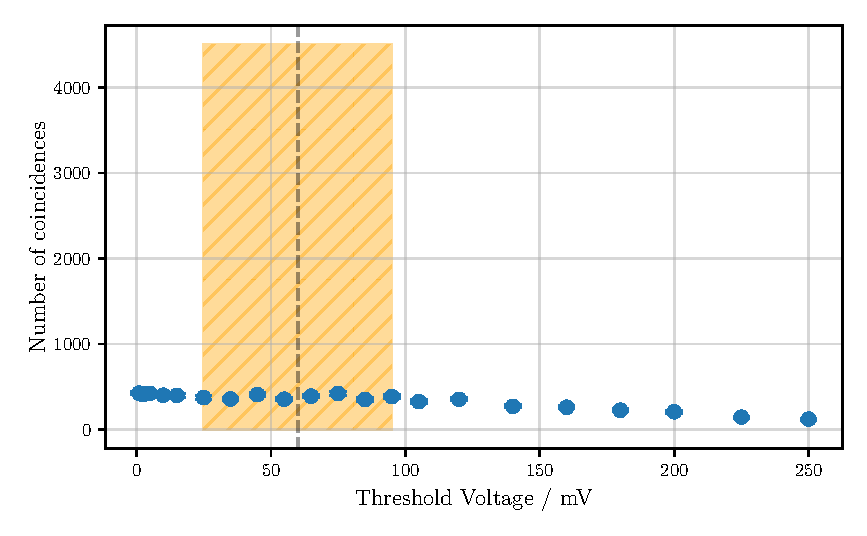
\includegraphics[width=\textwidth]{plots/threshL10_2.pdf}
        \captionof{figure}{Data of the second measurement of the \texttt{L10} PMTs.
        The central value of the plateau is $\SI{60}{mV}$.}
    \end{subfigure}\hfill
    \begin{subfigure}[b]{0.48\textwidth}
        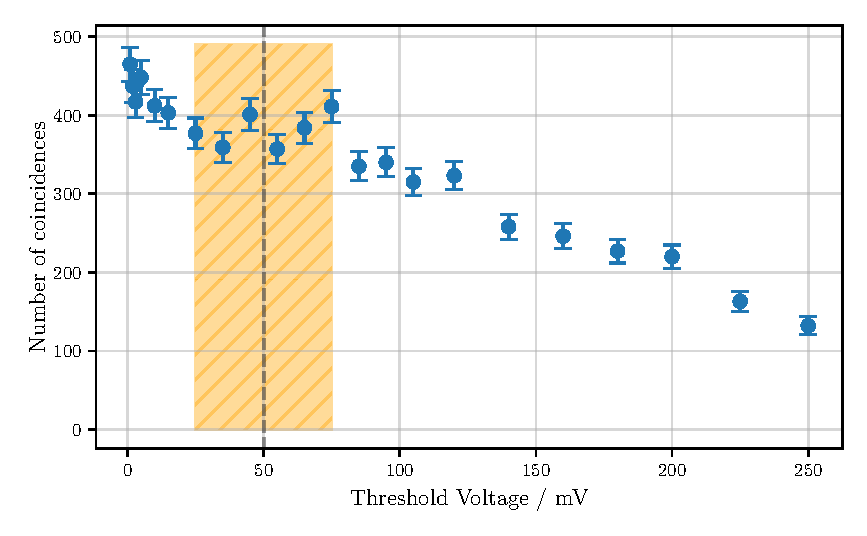
\includegraphics[width=\textwidth]{plots/threshL20.pdf}
        \captionof{figure}{Data of the \texttt{L20} PMTs.
        The central value of the plateau is $\SI{50}{mV}$.}
    \end{subfigure}
    \caption{Measured number of coincidences concerning varying threshold voltages
    of the \texttt{L10} and \texttt{L20} PMTs.
    The dashed line indicates the central values of each plateau. The striped orange areas mark the found plateaus.}
    \label{fig:appthresh5}
\end{figure}
\begin{figure}
    \centering
    \begin{subfigure}[b]{0.48\textwidth}
        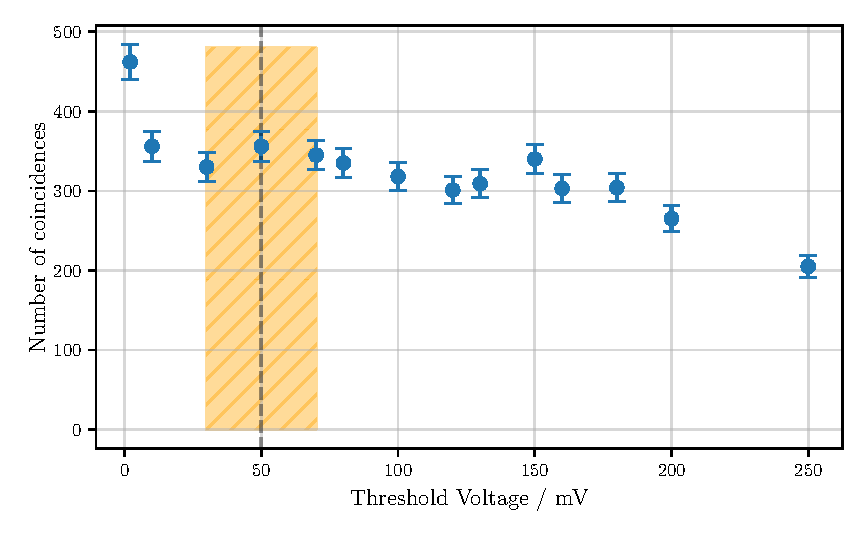
\includegraphics[width=\textwidth]{plots/threshL21.pdf}
        \captionof{figure}{Data of the \texttt{L21} PMTs.
        The central value of the plateau is $\SI{50}{mV}$.}
    \end{subfigure}\hfill
    \begin{subfigure}[b]{0.48\textwidth}
        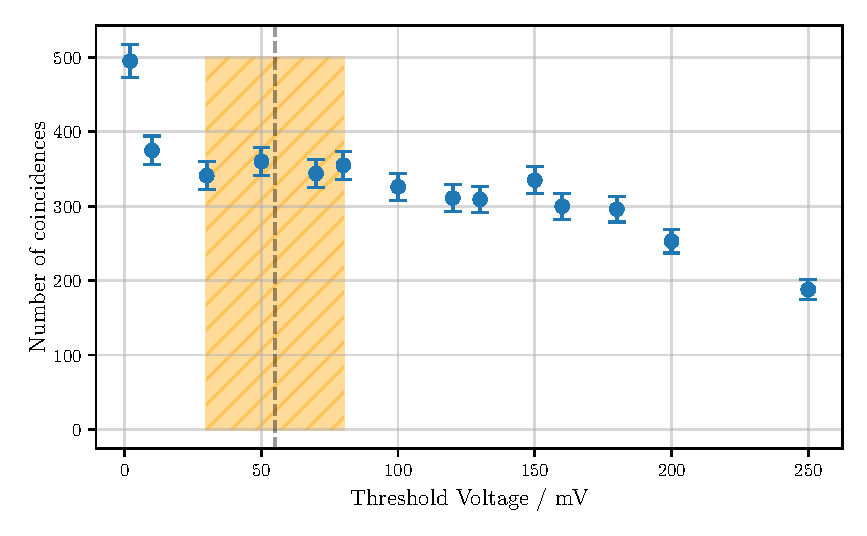
\includegraphics[width=\textwidth]{plots/threshR21.pdf}
        \captionof{figure}{Data of the \texttt{R21} PMTs.
        The central value of the plateau is $\SI{55}{V}$.}
    \end{subfigure}
    \caption{Measured number of coincidences concerning varying threshold voltages
    of the \texttt{L21} and \texttt{R21} PMTs.
    The dashed line indicates the central values of each plateau. The striped orange areas mark the found plateaus.}
    \label{fig:appthresh6}
\end{figure}

\chapter{TDC calibrations}
\label{sec:tdc_figures}
\begin{figure}
    \centering
    \begin{subfigure}[b]{0.48\textwidth}
        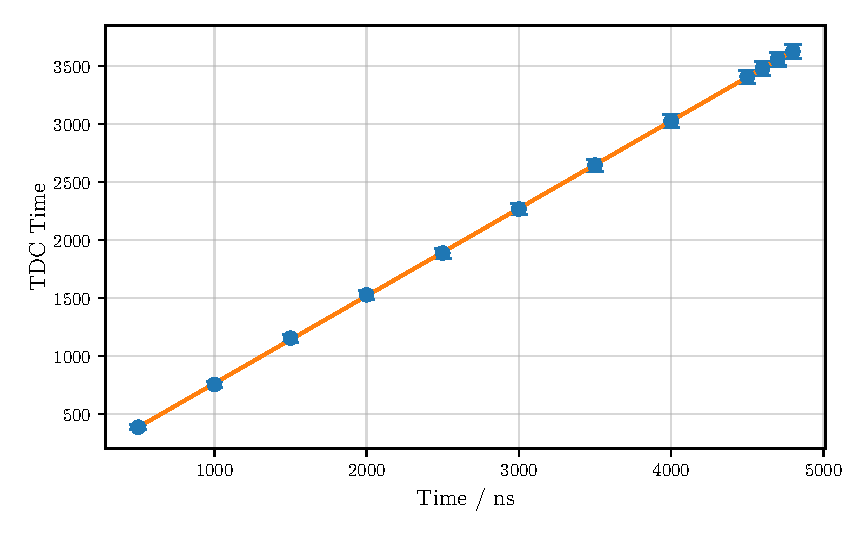
\includegraphics[width=\textwidth]{plots/tdc0.pdf}
        \captionof{figure}{TDC 1, Channel 1.}
    \end{subfigure}\hfill
    \begin{subfigure}[b]{0.48\textwidth}
        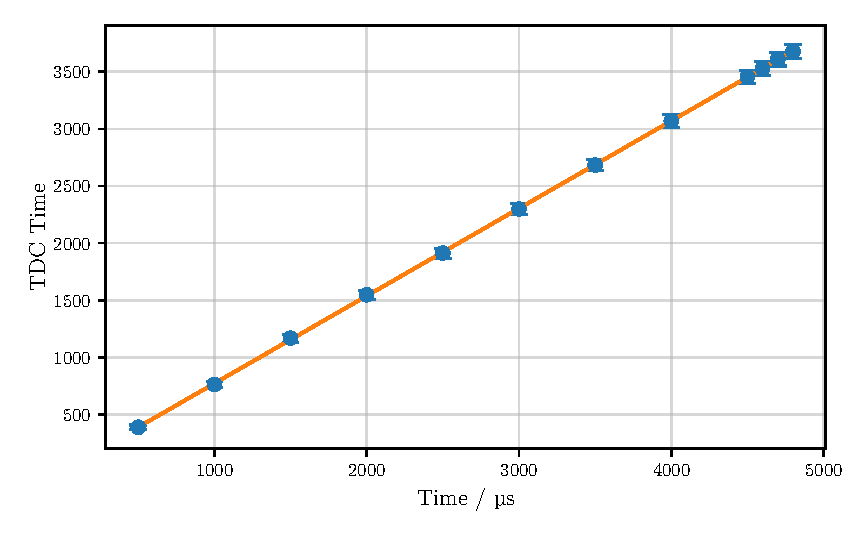
\includegraphics[width=\textwidth]{plots/tdc1.pdf}
        \captionof{figure}{TDC 1, Channel 2}
    \end{subfigure}
    \caption{Calibration Fits of Channel 1 and 2 of TDC 1.}
    \label{fig:tdc01}
\end{figure}
\begin{figure}
    \centering
    \begin{subfigure}[b]{0.48\textwidth}
        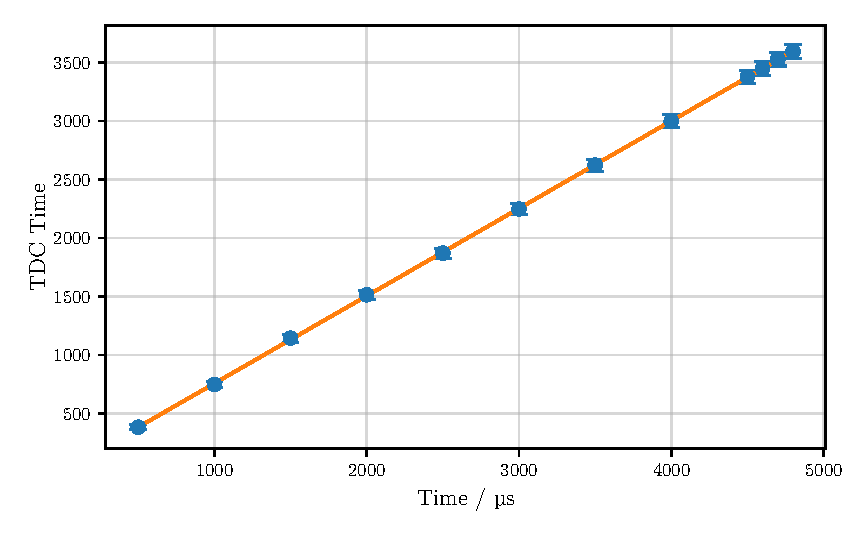
\includegraphics[width=\textwidth]{plots/tdc2.pdf}
        \captionof{figure}{TDC 1, Channel 3.}
    \end{subfigure}\hfill
    \begin{subfigure}[b]{0.48\textwidth}
        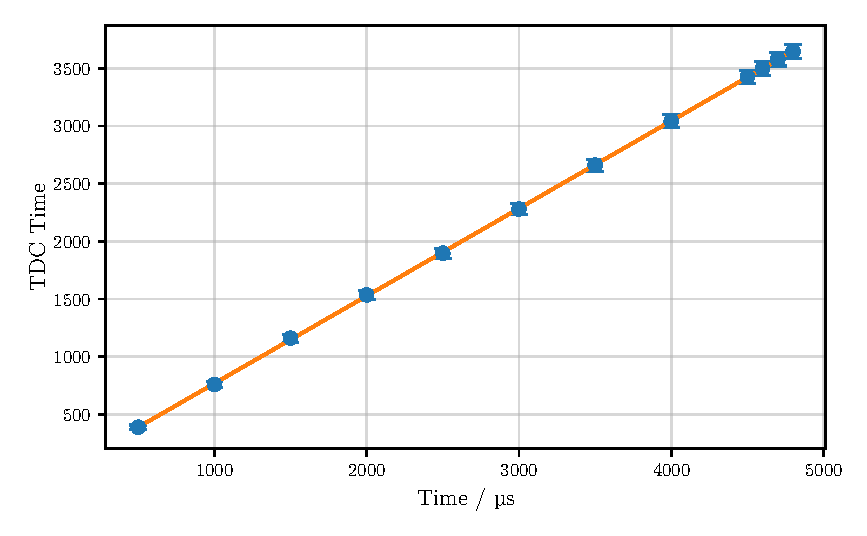
\includegraphics[width=\textwidth]{plots/tdc3.pdf}
        \captionof{figure}{TDC 1, Channel 4}
    \end{subfigure}
    \caption{Calibration Fits of Channel 3 and 4 of TDC 1.}
    \label{fig:tdc23}
\end{figure}
\begin{figure}
    \centering
    \begin{subfigure}[b]{0.48\textwidth}
        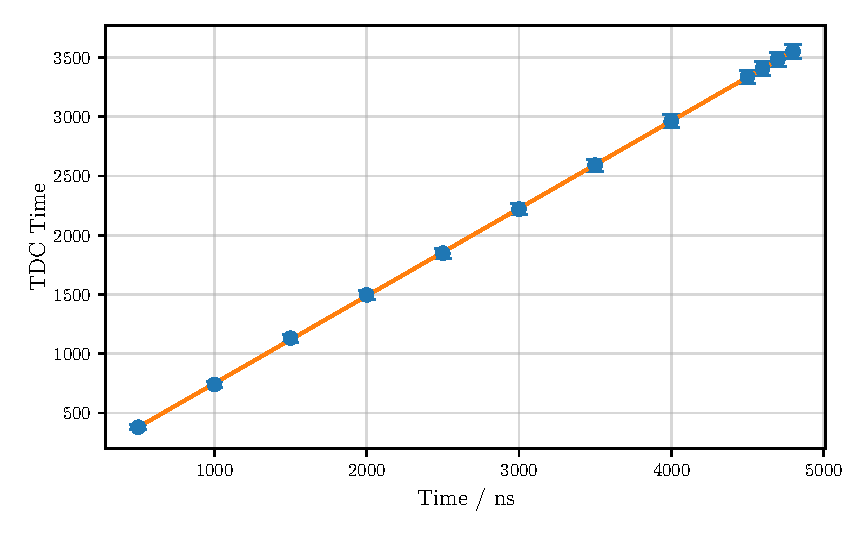
\includegraphics[width=\textwidth]{plots/tdc4.pdf}
        \captionof{figure}{TDC 1, Channel 5.}
    \end{subfigure}\hfill
    \begin{subfigure}[b]{0.48\textwidth}
        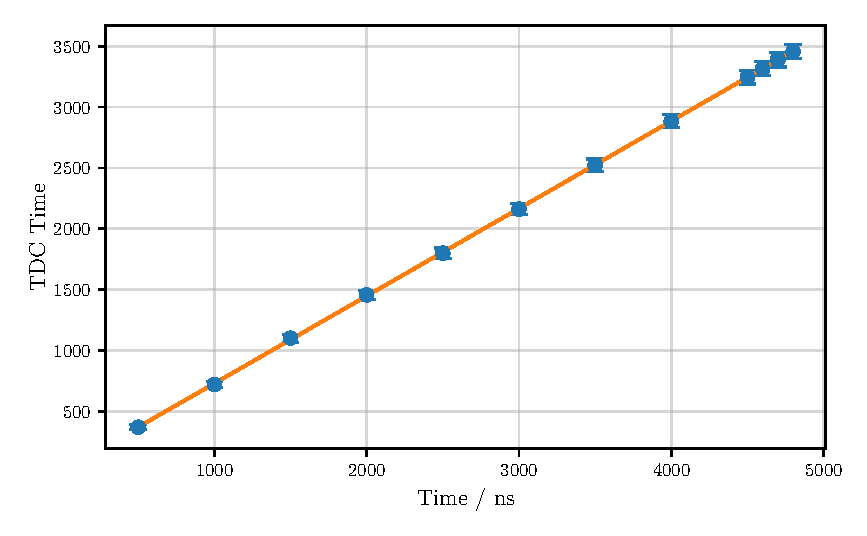
\includegraphics[width=\textwidth]{plots/tdc5.pdf}
        \captionof{figure}{TDC 1, Channel 6}
    \end{subfigure}
    \caption{Calibration Fits of Channel 5 and 6 of TDC 1.}
    \label{fig:tdc45}
\end{figure}
\begin{figure}
    \centering
    \begin{subfigure}[b]{0.48\textwidth}
        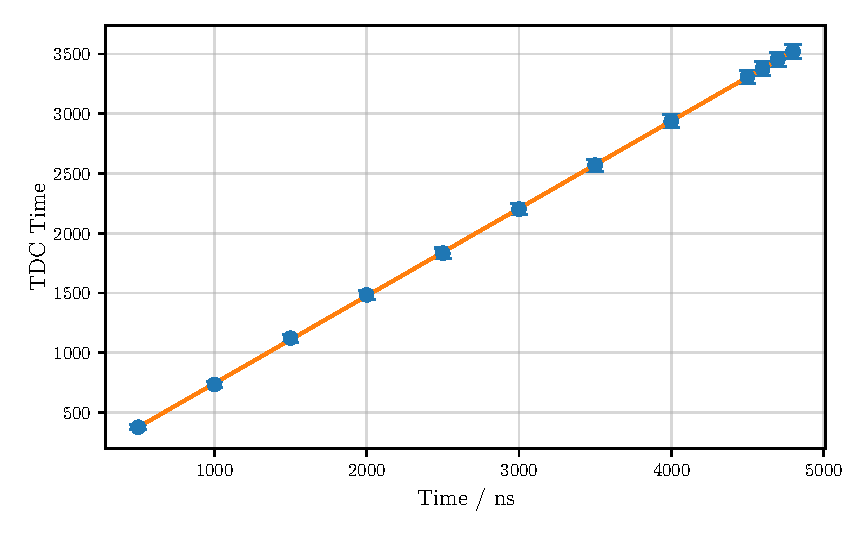
\includegraphics[width=\textwidth]{plots/tdc6.pdf}
        \captionof{figure}{TDC 1, Channel 7.}
    \end{subfigure}\hfill
    \begin{subfigure}[b]{0.48\textwidth}
        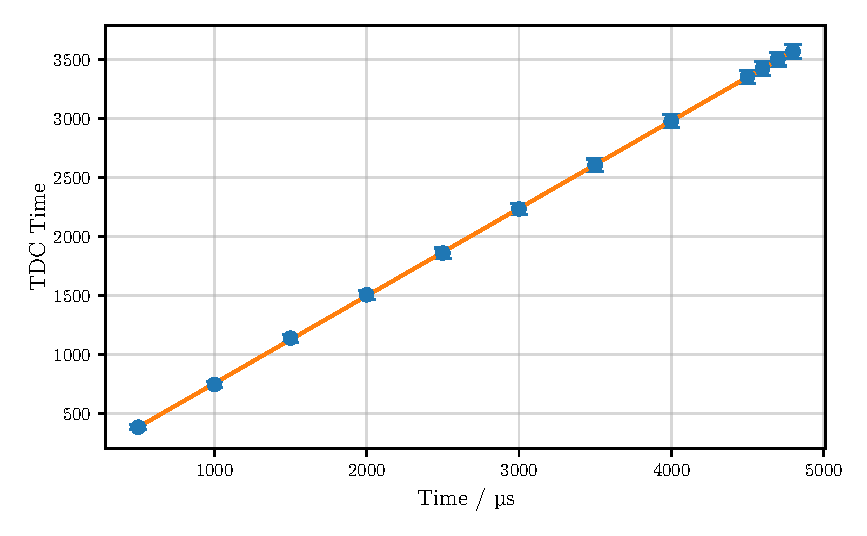
\includegraphics[width=\textwidth]{plots/tdc7.pdf}
        \captionof{figure}{TDC 1, Channel 8}
    \end{subfigure}
    \caption{Calibration Fits of Channel 7 and 8 of TDC 1.}
    \label{fig:tdc67}
\end{figure}

\begin{figure}
    \centering
    \begin{subfigure}[b]{0.48\textwidth}
        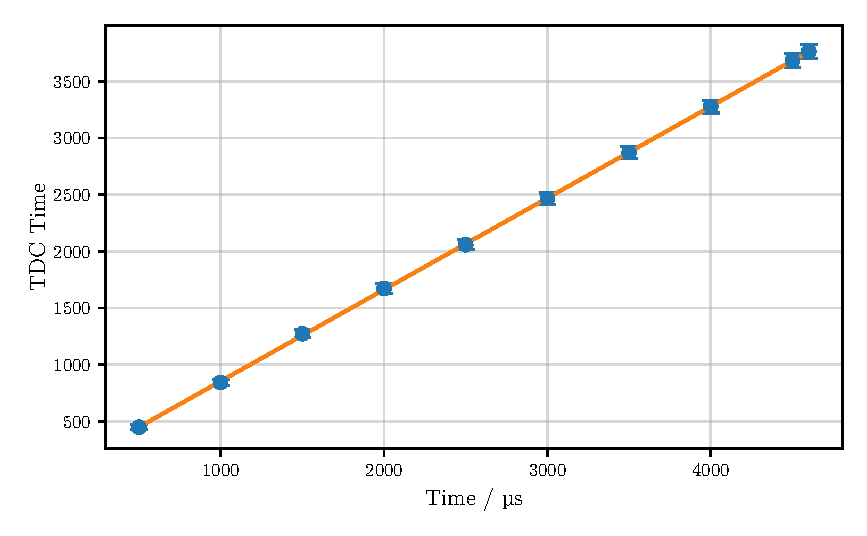
\includegraphics[width=\textwidth]{plots/tdc8.pdf}
        \captionof{figure}{TDC 2, Channel 1.}
    \end{subfigure}\hfill
    \begin{subfigure}[b]{0.48\textwidth}
        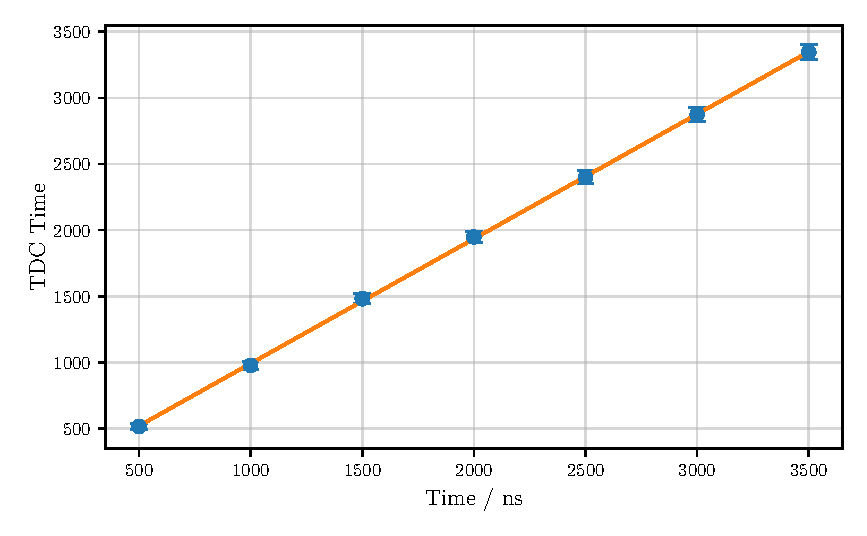
\includegraphics[width=\textwidth]{plots/tdc9.pdf}
        \captionof{figure}{TDC 2, Channel 2}
    \end{subfigure}
    \caption{Calibration Fits of Channel 1 and 2 of TDC 2. 
    Range of Channel 1 is limited to \SI{4.6}{\micro\second} and range of Channel 2 is limited to \SI{3.5}{\micro\second}.}
    \label{fig:tdc89}
\end{figure}
\begin{figure}
    \centering
    \begin{subfigure}[b]{0.48\textwidth}
        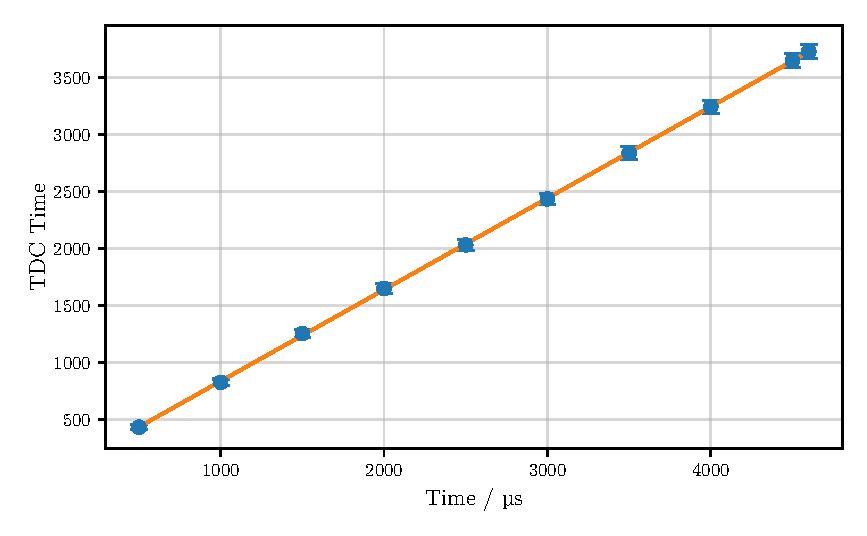
\includegraphics[width=\textwidth]{plots/tdc10.pdf}
        \captionof{figure}{TDC 2, Channel 3.}
    \end{subfigure}\hfill
    \begin{subfigure}[b]{0.48\textwidth}
        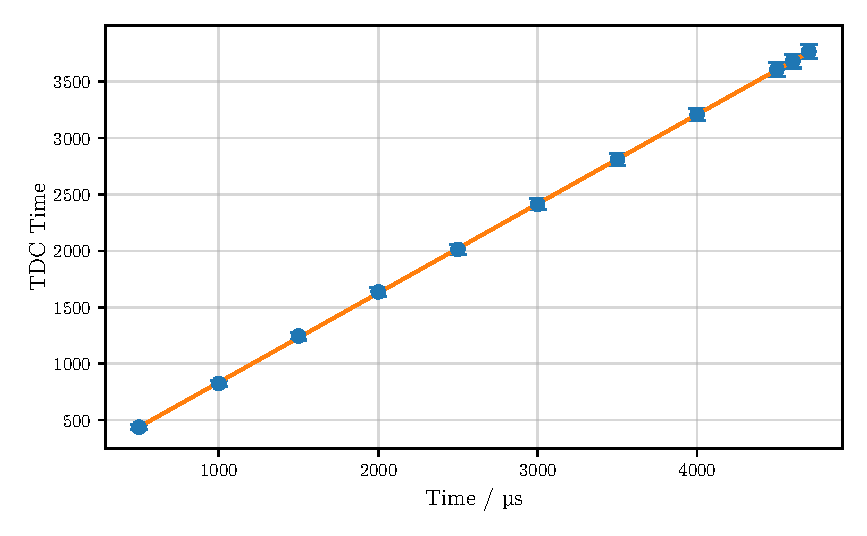
\includegraphics[width=\textwidth]{plots/tdc11.pdf}
        \captionof{figure}{TDC 2, Channel 4}
    \end{subfigure}
    \caption{Calibration Fits of Channel 3 and 4 of TDC 2. 
    Range of Channel 3 is limited to \SI{4.6}{\micro\second} and range of Channel 4 is limited to \SI{4.7}{\micro\second}.}
    \label{fig:tdc1011}
\end{figure}
\begin{figure}
    \centering
    \begin{subfigure}[b]{0.48\textwidth}
        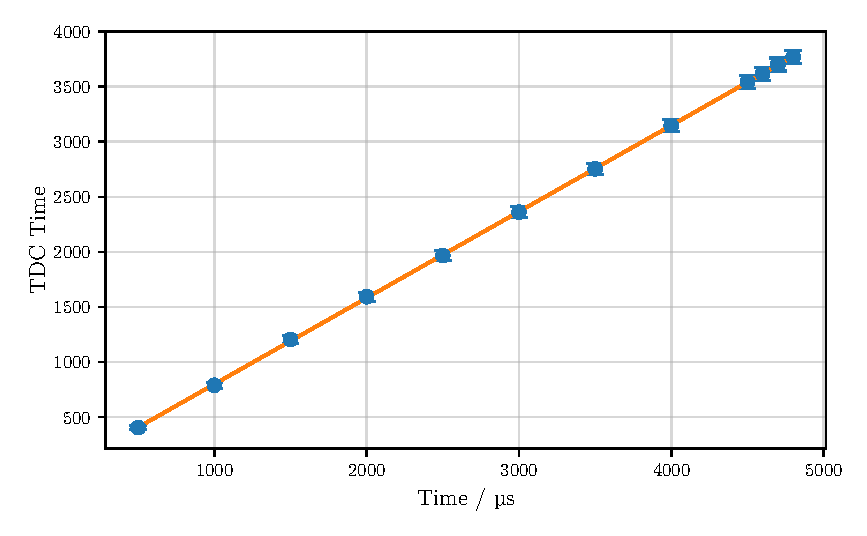
\includegraphics[width=\textwidth]{plots/tdc12.pdf}
        \captionof{figure}{TDC 2, Channel 5.}
    \end{subfigure}\hfill
    \begin{subfigure}[b]{0.48\textwidth}
        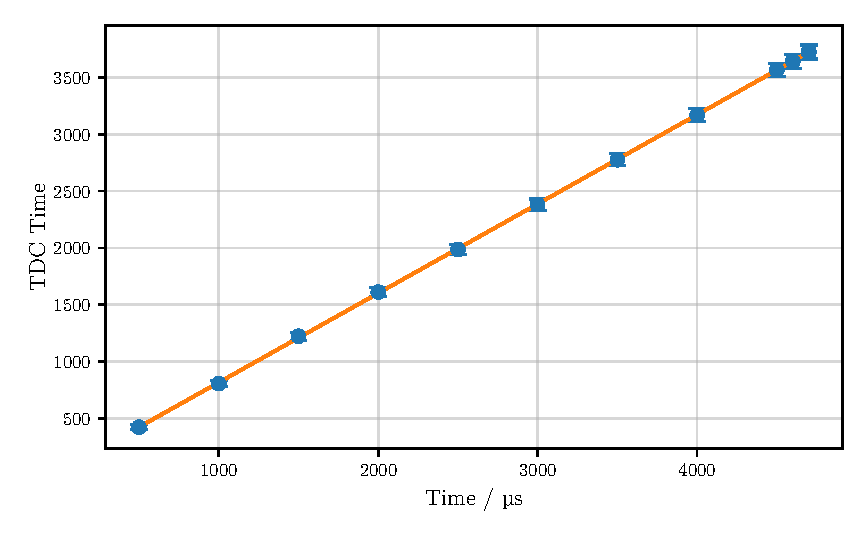
\includegraphics[width=\textwidth]{plots/tdc13.pdf}
        \captionof{figure}{TDC 2, Channel 6}
    \end{subfigure}
    \caption{Calibration Fits of Channel 5 and 6 of TDC 2. 
    Range of Channel 6 is limited to \SI{4.8}{\micro\second}.}
    \label{fig:tdc1213}
\end{figure}
\begin{figure}
    \centering
    \begin{subfigure}[b]{0.48\textwidth}
        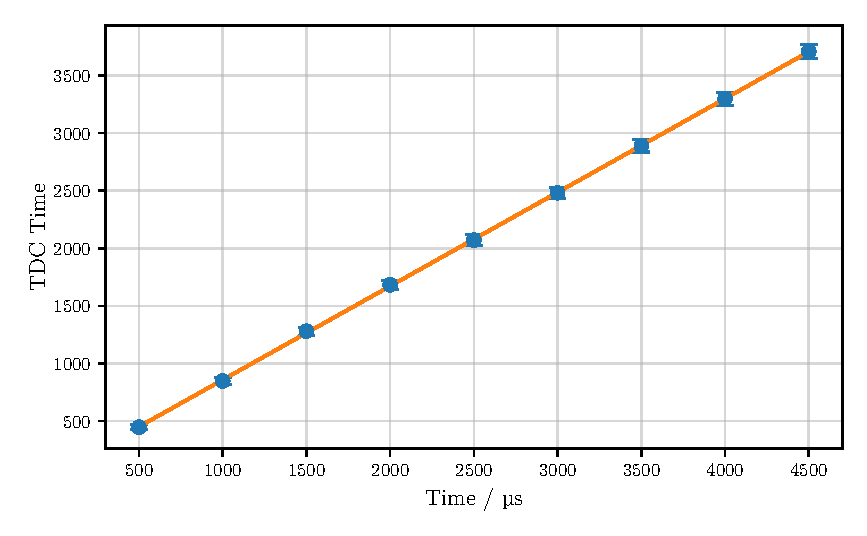
\includegraphics[width=\textwidth]{plots/tdc14.pdf}
        \captionof{figure}{TDC 2, Channel 7.}
    \end{subfigure}\hfill
    \begin{subfigure}[b]{0.48\textwidth}
        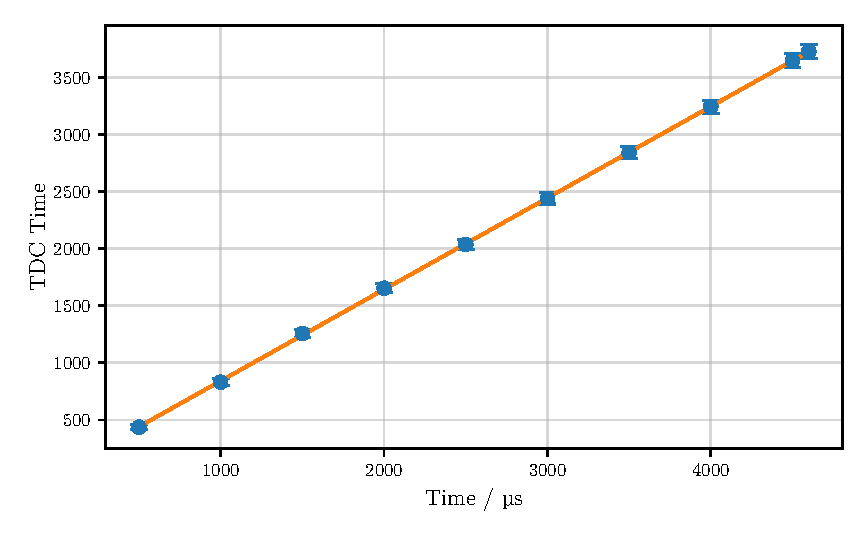
\includegraphics[width=\textwidth]{plots/tdc15.pdf}
        \captionof{figure}{TDC 2, Channel 8}
    \end{subfigure}
    \caption{Calibration Fits of Channel 7 and 8 of TDC 2. 
    Range of Channel 7 is limited to \SI{4.5}{\micro\second} and range of Channel 8 is limited to \SI{4.6}{\micro\second}.}
    \label{fig:tdc1415}
\end{figure}